% -*-cap2.tex-*-
% Este fichero es parte de la plantilla LaTeX para
% la realización de Proyectos Final de Carrera, protegido
% bajo los términos de la licencia GFDL.
% Para más información, la licencia completa viene incluida en el
% fichero fdl-1.3.tex

% Copyright (C) 2009 Pablo Recio Quijano 

\section{Introducción}

El primer paso que vamos a dar para describir el diseño de la aplicación será describir los requisitos del
sistema necesarios para poder ejecutar la aplicación, y posteriormente comentaremos las herramientas que se
van a usar para el desarrollo de la aplicación.

\section{Definición de los requisitos del sistema}

Los requisitos hardware y software necesarios para poder ejecutar con soltura la aplicación son los siguientes:

\begin{itemize}
	\item Sistema operativo Microsoft Windows en su versión Windows 7, o sistemas basados en GNU/Linux tales como
		la distribución Ubuntu en su versión 10.04.
	\item Últimas actualizaciones del sistema instaladas, drivers y demás aplicaciones propias del sistema
		configuradas correctamente.
	\item Procesador igual o superior a 1,6 GHz.
	\item Memoria RAM igual o superior a 512 MB
	\item Tarjeta gráfica con aceleración 3D con un mínimo de 128 MB
	\item En versiones basadas en Linux, se requieren las siguientes librerías:
		\begin{itemize}
			\item python-pygame
			\item python-setuptools
			\item PyOpenGL
			\item PyOpenGL-accelerate
		\end{itemize}
	\item Por otro lado, si el sistema está basado en Microsoft Windows, necesitaremos:
		\begin{itemize}
			\item Pygame
			\item Python OpenGL and Gloss
		\end{itemize}
\end{itemize}

\section{Herramientas utilizadas}

\subsection{Librería gráfica}

Para todo el tema del aspecto gráfico, mi tutor me recomendó que utilizara las librerías SDL\footnote{Simple
Directmedia Layer}, ya que son unas librerías orientadas al desarrollo de videojuegos con varias particularidades:
\begin{itemize}
    \item Son completas, ya que permiten gestionar operaciones de dibujo en dos dimensiones, efectos de
            sonido y música, carga y gestión de imágenes, subsistemas de control de métodos de entrada,
            etcétera, por lo que contamos con una solución global para desarrollar videojuegos.
    \item Están programas en C, por lo que se puede esperar un buen rendimiento de las librerías en
            diferentes entornos.
    \item Multiplataforma: es compatible oficialmente con los sistemas Microsoft Windows, GNU/Linux,
            Mac OS y QNX, además de otras arquitecturas y sistemas menos comunes como Sega Dreamcast, Sony PSP,
            WebOS, Google Android o Symbian entre otros.
    \item Tampoco hay que mantener al margen la característica de que cuenta con wrappers a otros lenguajes
            de programación como entre los que se encuentran C++, Ada, C\#, BASIC, Erlang, Lua, Java o Python, por
            lo que nos da bastante libertad para elegir un lenguaje de programación principal
    \item Publicado bajo licencia LGPL, con todas las ventajas que conlleva.
    \item Y por último no hay que menospreciar que mi tutor emplea SDL a la hora de impartir la asignatura
            de diseño de videojuegos, y contar con esa base de conocimiento nos ayudará a desarrollar más rápidamente
            y solucionar antes nuestros posible problemas.
\end{itemize}

\begin{figure}[h]
  \label{logo-sdl}
  \begin{center}
    
\includegraphics[scale=0.5]{SDL.png}
  \end{center}
  \caption{Logotipo de la librería Simple DirectMedia Layer}
\end{figure}

En este aspecto, la utilización de las librerías SDL estaba clara. Potencia, comodidad, multiplataforma y con la posibilidad
de utilizar diferentes lenguajes de programación.\\

\subsection{Lenguaje de programación}

Una vez que tocamos el tema de los lenguajes de programación, entra en escena la problemática sobre qué lenguaje
utilizar. En principio se pensó emplear el lenguaje C++ por dos sencillas razones:

\begin{enumerate}
    \item Por un lado es un lenguaje que hemos aprendido en la carrera, se ha utilizado en varias asignaturas de
            diferentes ramas, con lo cual la comodidad y familiaridad que podemos tener a la hora de programar
            es un punto importante a tener en cuenta.
    \item Tampoco podemos olvidar que, al ser un lenguaje compilado, la velocidad de ejecución que se consigue
            es interesante, y mucho más tratándose de temas como la inteligencia artificial (donde puede ser
            necesario un uso intensivo de los recursos del sistema) o el desarrollo de videojuegos (en el que
            la potencia del ordenador repercute en una mejor experiencia del usuario)
\end{enumerate}

Pero hay que detenerse un momento y pensar en la naturaleza del proyecto. Aunque el programa a desarrollar sea un
videojuego, no hay que olvidar que hay diferentes tipos de juegos, que pueden condicionar o influir en nuestra forma
de programarlo. En el caso del dominó, lo primero que debemos tener en cuenta es que el apartado gráfico no va a
requerir de una gran potencia o despliegue de efectos: el dominó es un juego pausado y a diferencia de otros
videojuegos lo importante en este caso es mostrar al usuario la información de la partida de una forma clara y sencilla,
para que el jugador evalúe las posibilidades de acción y actúe en consecuencia.\\

Si tenemos en cuenta estas circunstancias, existen otros lenguajes que también deben entrar en juego,
como por ejemplo \textbf{Python}. Buscando las diferencias, ventajas y desventajas de Python frente a C++,
obtenemos el siguiente listado:

\begin{enumerate}
    \item Python es un lenguaje de programación multiparadigma ya que soporta orientación a objetos,
            programación imperativa y, en menor medida, programación funcional.
    \item Al igual que C++ es multiplataforma, y está publicado con la licencia \textbf{Python Software Foundation
            License}, que es una licencia de software libre permisiva, compatible con la GPL.
    \item La sintaxis de Python es muy clara, simple, expresiva y legible, con lo cual los programas
            desarrollados bajo Python son más sencillos de entender \cite{Pilgrim:2004:DP:983200}.
    \item Python es un lenguaje interpretado, a diferencia de C++ que es compilado. Este aspecto podría suponer una
            desventaja ya que al ser interpretado puede resultar más lento, pero analicemos pausadamente estos
            factores:
        \begin{itemize}
            \item Como ya hemos comentado previamente, nuestra aplicación, a pesar de enmarcarse dentro de las
                    facciones de un videojuego, no requiere de grandes alardes de potencia gráfica como podría
                    suponerse, ya que es un tipo de juego pausado y donde cómo se muestra la información
                    es mucho más importante que la velocidad o los efectos de vídeo e imágenes.
            \item A pesar de ser interpretado, un gran conjunto de las funcionalidades de python --- como librerías o
                    funciones básicas del lenguaje --- están programadas internamente en C, así que podríamos
                    verlo como que estamos utilizando la comodidad de Python sobre la potencia de C, uniendo
                    lo mejor de ambos mundos.
        \end{itemize}
\end{enumerate}

\subsection{Diseño y estilo visual de interfaces}

El diseño visual que se ha desarrollado para la interfaz se ha creado desde cero, buscando los siguientes objetivos:
\begin{itemize}
    \item Líneas sencillas, minimalistas, sin recargar innecesariamente la pantalla
    \item Botones grandes, para que sea fácil de utilizar por usuarios de edad avanzada.
    \item Textos con un punto de letra elevado, facilitando la rápida lectura y legibilidad del texto.
\end{itemize}

\begin{figure}[h]
  \label{interfaz}
  \begin{center}
    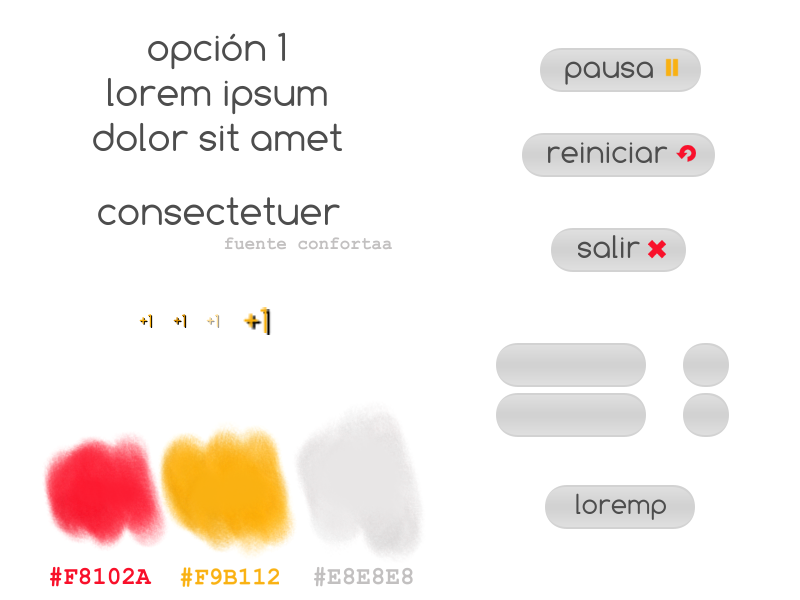
\includegraphics[scale=0.5]{ui.png}
  \end{center}
  \caption{Diferentes elementos utilizados en la interfaz}
\end{figure}

\subsection{Documentación del código}

Por otro lado, para gestionar toda la documentación del proyecto se decidió utilizar las siguientes herramientas:
\begin{itemize}
    \item \LaTeX\ para escribir la memoria, ya que es una forma robusta y fiable de escribir una memoria para
            un Proyecto Fin de Carrera, descartándose otras posibles opciones por no ser adecuadas para la escritura
            de un documento de estas características. Para facilitar la compilación dispone de la herramienta
            GNU Make~\cite{pdf:make}.
    \item Doxygen para la documentación del código fuente, porque además de documentar de manera sencilla y fácil
            de leer el mismo código fuente, genera una documentación en diferentes formatos. Además,
        \begin{itemize}
            \item Doxygen funciona con lenguajes como C++, C, Java, Objective-C, Python, Fortran, VHDL, PHP o C\#
                    (entre otros), por lo que se puede acomodar a nuestras necesidades. Incluso existe una
                    herramienta llamada \textbf{Doxypy} que nos permite reutilizar los comentarios \emph{tipo Python}
                    y adaptarlos a Doxygen, con lo cual ahorramos trabajo y cumplimos con la normativa
                    de código Python.
        \end{itemize}
\end{itemize}

\subsection{Sistema de control de versiones}

El código del proyecto Dominous, está alojado por completo dentro del sistema que proporciona Rediris, que básicamente
consiste en un entorno completo basado en Subversion -- SVN. \\ 

Subversion permite llevar un control exahustivo de todos los ficheros e iteraciones de código que se realizan en él,
permitiendo volver a versiones anteriores de código, comprobar diferencias entre versiones o ficheros y cualquier otra
operación propia de un sistema de control de versiones. \\

Se evaluaron otros sistemas de control de versiones distribuidos como GIT, Bazaar o Mercurial, pero se desecharon
básicamente porque, por un lado, este proyecto cuenta únicamente con un desarrollador, y multitud de ventajas que
ofrecen los sistemas de control de versiones distribuidos dejan de tener sentido, si tenemos en cuenta esta circunstancia
del proyecto, y por otro lado la integración de SVN con Rediris (con las ventajas de visualización de código y versiones
que ofrece ViewCVS) decantaron la decisión sobre el lado de SVN.

\section{Interfaz gráfica}

Tomando los resultados obtenidos en la fase de análisis es necesario diseñar una interfaz gráfica amigable
para el usuario y desde la cual se pueda interactuar con la aplicación. Para el diseño de las interfaces
se intentará en todo momento que sean usables además de intentar conseguir que el usuario no pueda
introducir datos erróneas para que no produzca comportamientos anómalos. \\

\begin{figure}[h]
  \label{fig:pantallas_interfaz}
  \begin{center}
    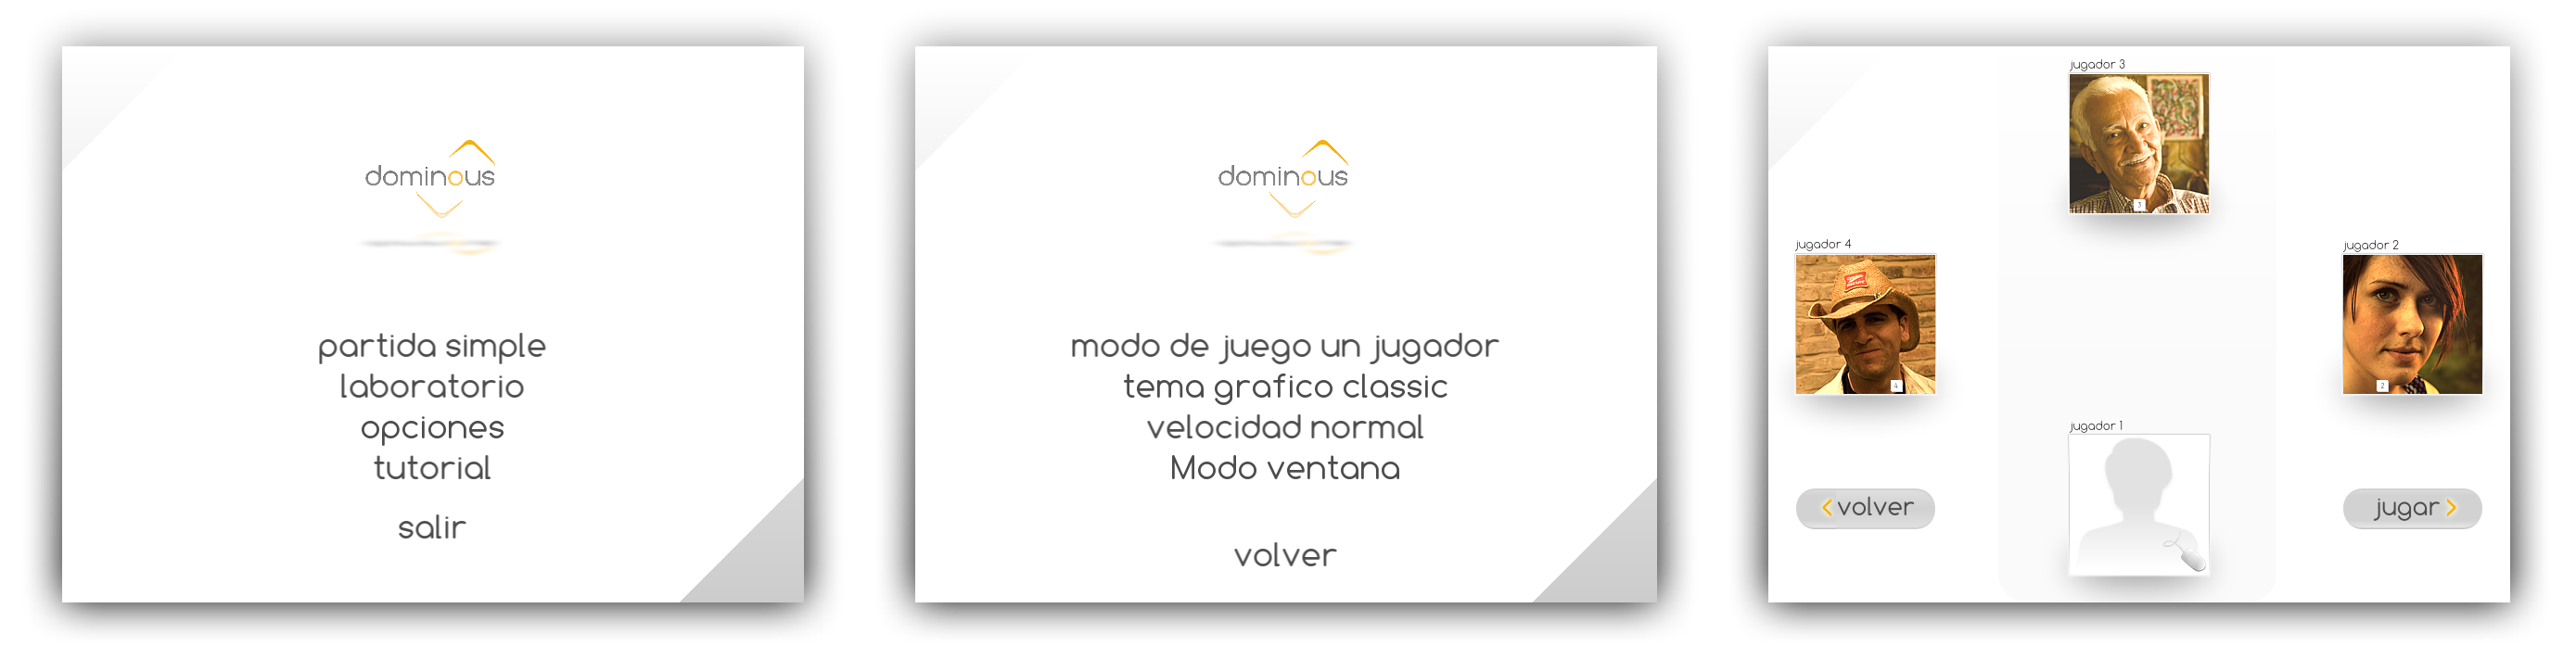
\includegraphics[scale=0.25]{interfaz.png}
  \end{center}
  \caption{Varias pantallas con la interfaz de Dominous}
\end{figure}

\subsection{Diagrama de interacción entre interfaces gráficas}

En el siguiente diagrama~\ref{fig:diagramainteraccioninterfaces} podemos observar la interacción entre
las distintas interfaces gráficas desarrolladas para la aplicación. \\

\begin{figure}[h]
  \label{fig:diagramainteraccioninterfaces}
  \begin{center}
    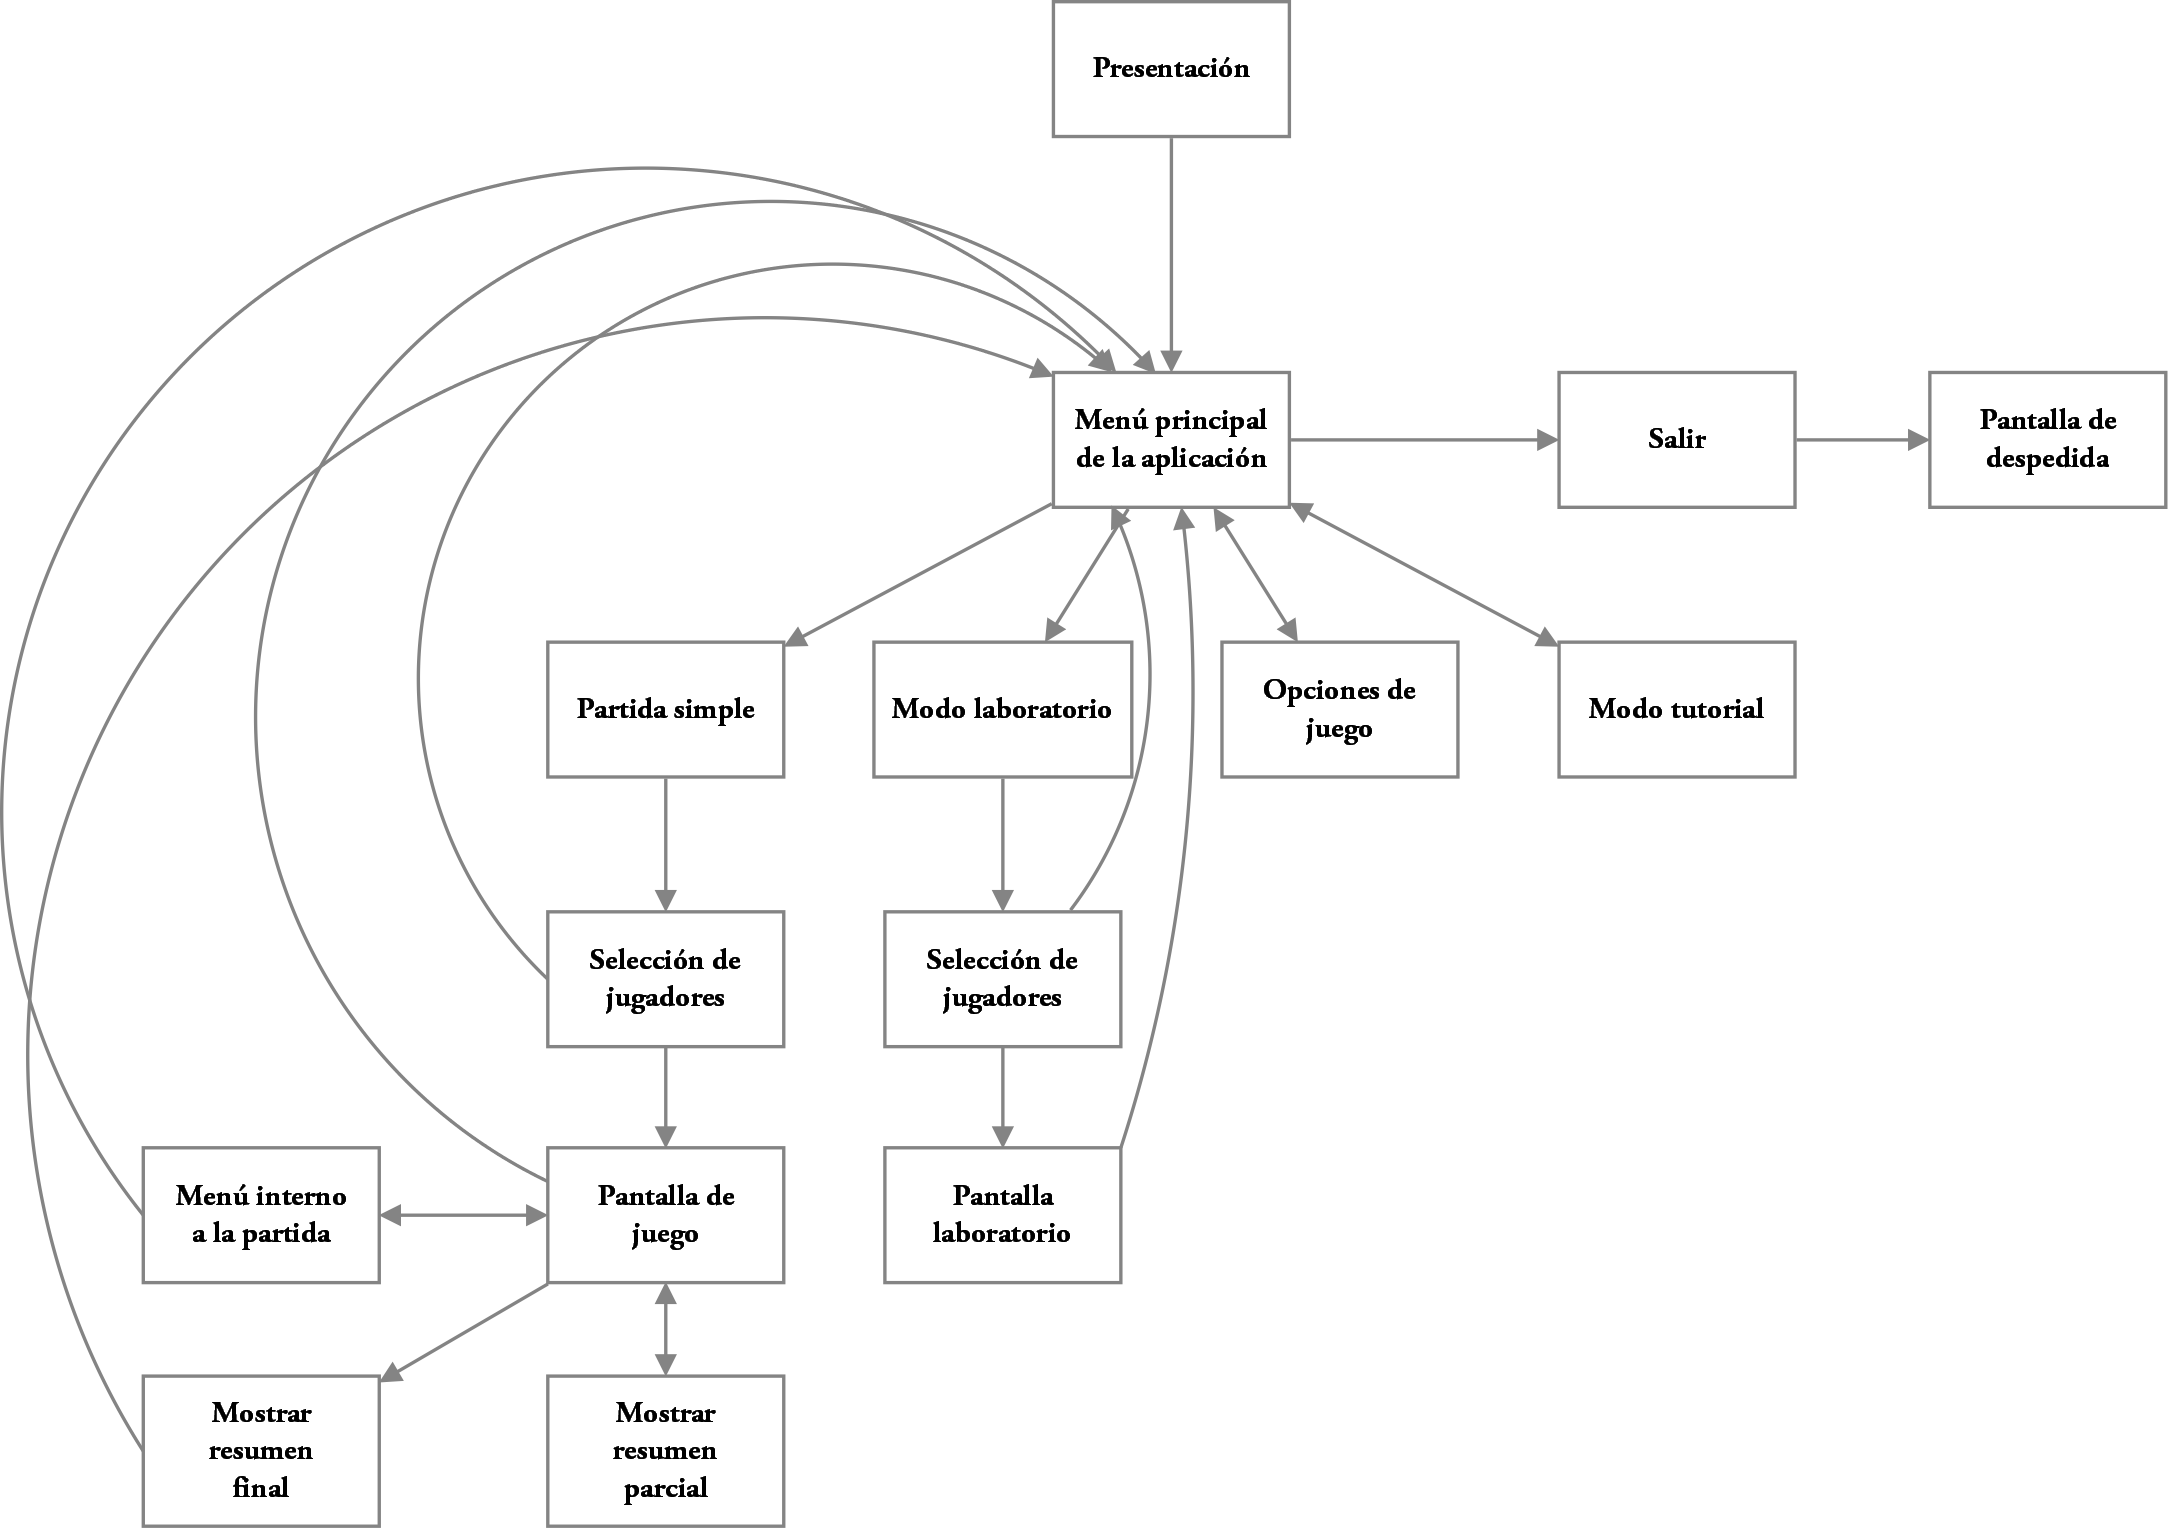
\includegraphics[scale=0.15]{diagrama_interfaces.png}
  \end{center}
  \caption{Diagrama de interacción entre interfaces}
\end{figure}

\section{Diagrama Entidad -- Relación}

La aplicación \textbf{Dominous} realiza un almacenamiento limitado de información, por lo que no se estima necesario
realizar un diagrama Entidad -- Relación con este fin.

\section{Diagrama de clases de diseño}



\section{Sistemas expertos}


